% visualisierung.tex
Wird der \texttt{visualize}-Parameter bei der Ausführung einer R-Paket-Funktion auf \texttt{TRUE} gesetzt, wird ein \texttt{RMarkdown}-Skript ausgeführt. Dieses generiert eine  Präsentation vom \LaTeX -Dokumenttyp \emph{Beamer} mit Informationen und Visualisierungen zur ausgeführten Funktion.
\\
Die erzeugten Präsentationen liegen innerhalb des Programmverzeichnisses von R im Installationsordner des Pakets. Dort gibt es den Ordner \emph{pdf}, in dem sich die Dokumente befinden. Möchte man die Dokumente von RStudio aus öffnen, anstatt die Dokumente in der Verzeichnisstruktur suchen zu müssen, kann die \texttt{ConvOpenPDF}-Funktion (siehe Funktion~\ref{funktion:ConvOpenPDF}) verwendet werden. Möchte man die Dokumente zu einem späteren Zeitpunkt erneut einsehen, wird empfohlen eine Kopie der Datei abzuspeichern, da bei einer erneuten Ausführung der gleichen Funktion inklusive Visualisierung das zuvor erzeugte Dokument im \emph{pdf}-Ordner überschrieben wird. Die vom \texttt{RMarkdown}-Skript erzeugten \LaTeX -Dateien, aus denen die Beamer Präsentationen generiert werden, liegen ebenfalls im selben Verzeichnis.
\\
Da einerseits der Platz auf einer Folie begrenzt ist und andererseits Visualisierungen zu Lehrzwecken nur für kurze Bitsequenzen sinnvoll sind, gibt es Einschränkungen für die in einer Visualisierung verwendeten Nachrichten und Kodierer. Eine Visualisierung der Kodierung bzw. Dekodierung erfolgt für Nachrichten bzw. dekodierte Nachrichten inklusive Terminierungsbits bei einer Länge von bis zu 14 Bits. Bei einem Faltungskodierer mit einer Schieberegisterlänge von vier oder größer erfolgt keine Visualisierung der Dekodierung, da das Trellis zu groß ist. Bei der Kodierung wird nur das Zustandsdiagramm nicht abgebildet.

Bei den folgenden Beispielen der Visualisierungen wurde stets punktiert, da ohne Punktierung die Informationen zur Punktierung in den Präsentationen fehlen und somit auch nicht erläutert werden können.

Der weitere Kapitelinhalt setzt sich folgendermaßen zusammen: Die Kapitel~\ref{kapitel:visualisierung_kodierung} bzw. \ref{kapitel:visualisierung_dekodierung} beinhalten Erläuterungen zur Visualisierung der Kodierung bzw. Dekodierung. Kapitel~\ref{kapitel:visualisierung_simulation} beschreibt die Visualisierung der Simulation.
\section{Kodierung}
\label{kapitel:visualisierung_kodierung}
% allg. Informationen
Bei der Kodierung befinden sich auf den ersten Folien allgemeine Informationen zum verwendeten Faltungskodierer. Abbildung~\ref{abb:folie_kodierer_kennwerte} zeigt die Folie mit den Kennwerten des Faltungskodierers: Anzahl an Ausgängen $N$, Länge des Schieberegisters $M$, Generatorpolynome, Punktierungsmatrix und Koderate. Auf den nächsten beiden Folien werden die Zustandsübergangsmatrix und die Ausgabematrix abgebildet. In Abbildung~\ref{abb:folie_zustandsübergangsmatrix} ist die Folie der Zustandsübergangsmatrix zu sehen. Analog dazu wird die Ausgabematrix auf der nächsten Folie veranschaulicht. Diese wird aus Platzgründen hier nicht abgebildet.
\begin{figure}[th]
	\centering
	\begin{subfigure}{0.48\textwidth}
		\centering
		\fbox{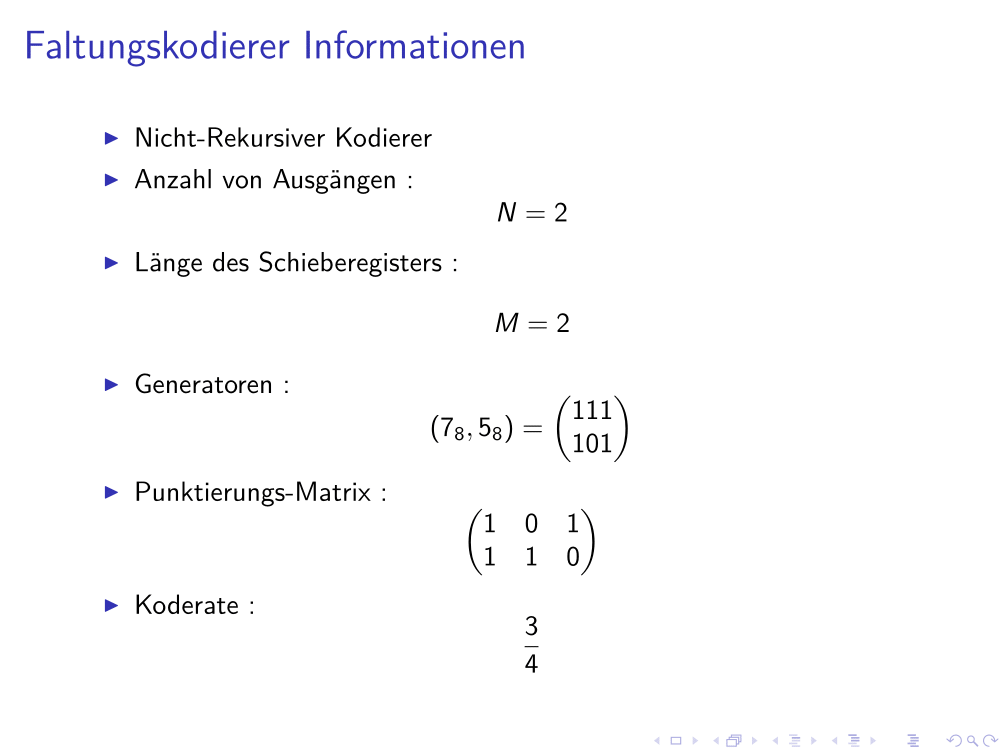
\includegraphics[width=0.99\textwidth]{abbildungen/folie_kodierung_info}}
		\caption{Folie mit Kodierer-Kennwerten}
		\label{abb:folie_kodierer_kennwerte}
	\end{subfigure}
	\quad % spacing between subfigures
	\begin{subfigure}{0.48\textwidth}
		\centering
		\fbox{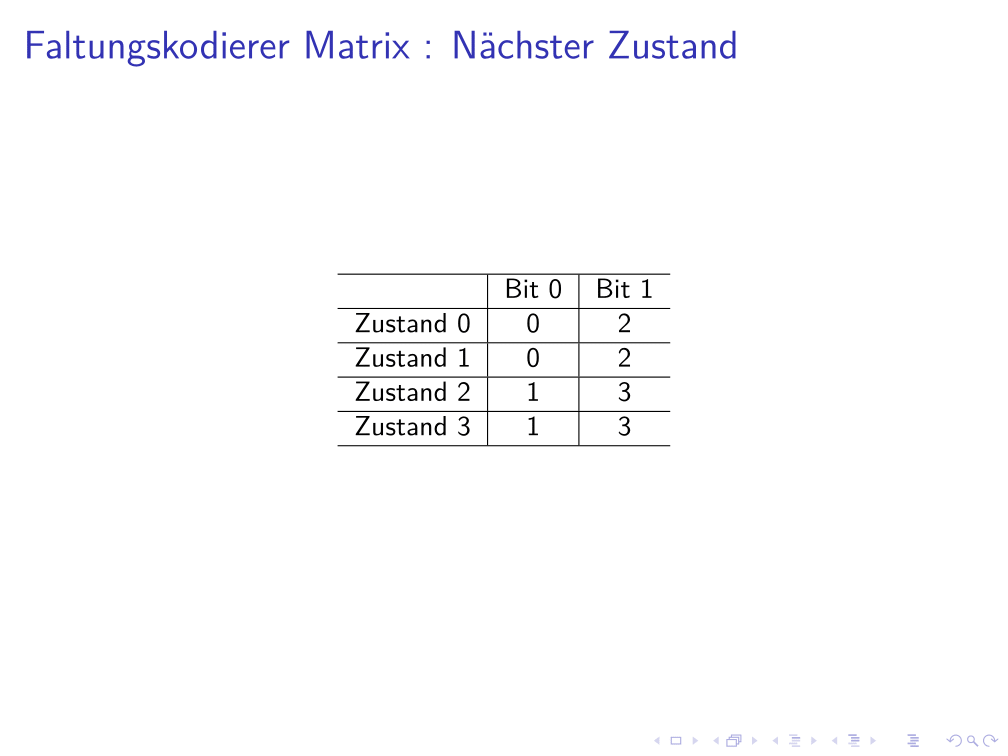
\includegraphics[width=0.99\textwidth]{abbildungen/folie_kodierung_matrix_zustand}}
		\caption{Folie mit Zustandsübergangsmatrix}
		\label{abb:folie_zustandsübergangsmatrix}
	\end{subfigure}
	\caption{Folien mit allgemeinen Informationen zum Faltungskodierer}
	\label{abb:folie_allg_info_kodierer}
\end{figure}
% Kodierung
Anschließend folgt die Visualisierung der Kodierung. Dabei wird die zu kodierende Nachricht Bit für Bit auf einer eigenen Folie verarbeitet. Abbildung~\ref{abb:folie_kodierung} zeigt die ersten beiden Schritte sowie den letzten Schritt der Kodierung. In Abbildung~\ref{abb:folie_kodierung_1} ist die Folie vor der Kodierung des ersten Bits zu sehen. Zunächst ist die zu kodierende Nachricht (Input), das Zustandsübergangsdiagramm, sowie eine noch nicht befüllte Kodierungstabelle zu sehen. Das Kodewort wird auf den folgenden Folien Schritt für Schritt erarbeitet. Durch diese Herangehensweise ist die Kodierung für den Benutzer einfach nachzuvollziehen. Abbildung~\ref{abb:folie_kodierung_2} zeigt die Folie der Kodierung des ersten Bits. Das erste Bit des Inputs, der aktuelle Zustand, der Folgezustand sowie der resultierende Output werden in eine neue Zeile der Kodierungstabelle geschrieben. Der aktuelle Zustand sowie der entsprechende Übergang werden im Diagramm farblich hervorgehoben, um die Kodierung auch im Zustandsdiagramm verfolgen zu können. Der Output wird auch unterhalb der Tabelle eingetragen und wächst mit jedem Schritt bis schlussendlich die gesamte Nachricht kodiert wurde. Die Visualisierung am Ende der Kodierung ist in Abbildung~\ref{abb:folie_kodierung_3} zu sehen. Die Bits unterhalb der horizontalen Trennlinie in der Tabelle stellen die Terminierungsbits dar.
\begin{figure}[th]
	\centering
	\begin{subfigure}{0.48\textwidth}
		\centering
		\fbox{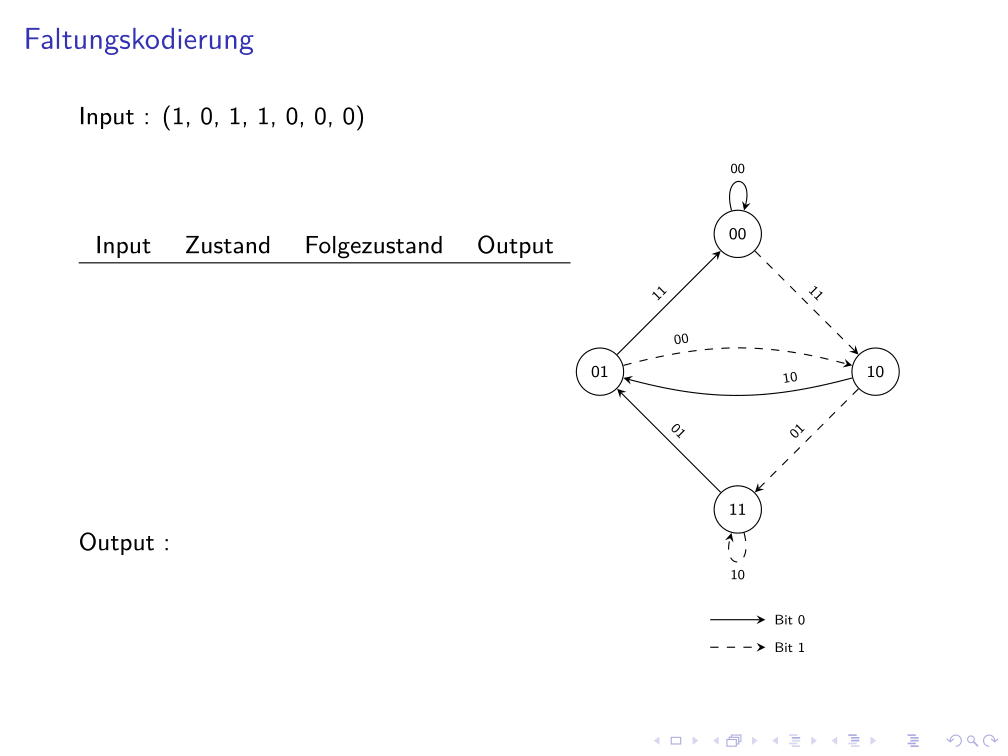
\includegraphics[width=0.99\textwidth]{abbildungen/folie_kodierung_1}}
		\caption{}
		\label{abb:folie_kodierung_1}
	\end{subfigure}
	\quad
	\begin{subfigure}{0.48\textwidth}
		\centering
		\fbox{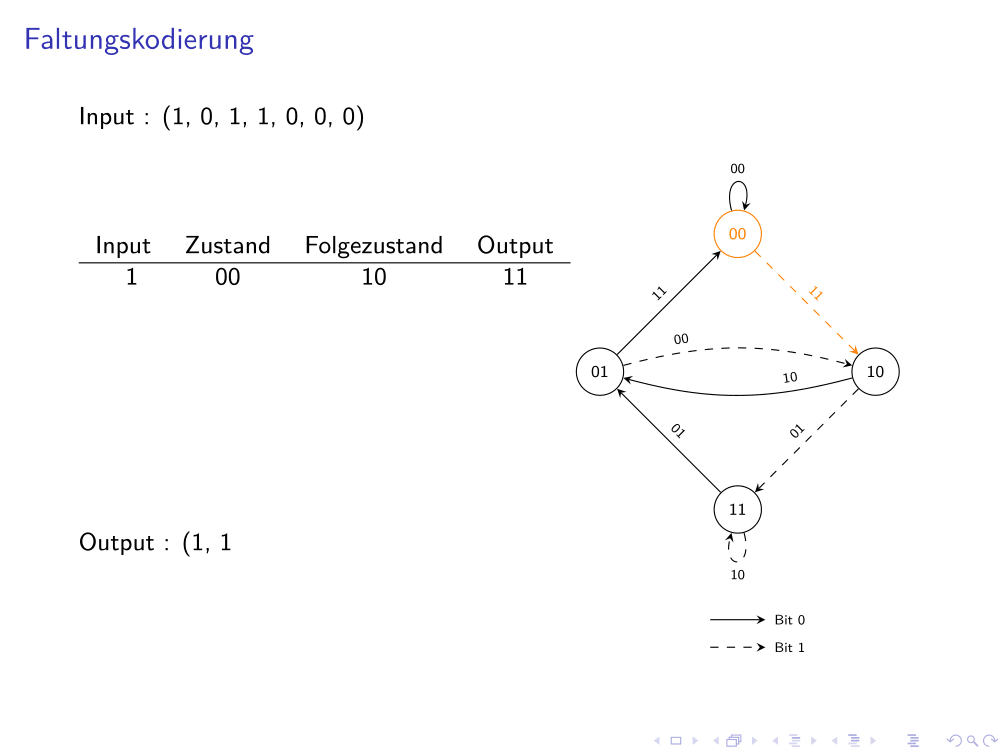
\includegraphics[width=0.99\textwidth]{abbildungen/folie_kodierung_2}}
		\caption{}
		\label{abb:folie_kodierung_2}
	\end{subfigure}
	\par\bigskip
	\begin{subfigure}{0.7\textwidth}
		\centering
		\fbox{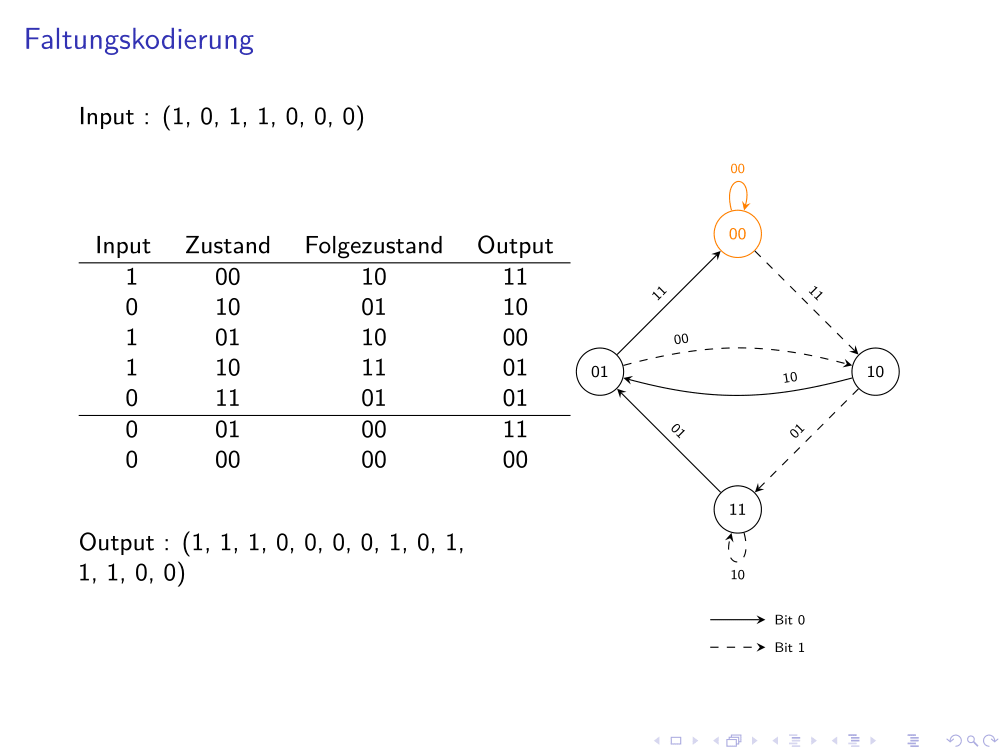
\includegraphics[width=0.99\textwidth]{abbildungen/folie_kodierung_3}}
		\caption{}
		\label{abb:folie_kodierung_3}
	\end{subfigure}
	\caption{Folien der Kodierung}
	\label{abb:folie_kodierung}
\end{figure}
% Kode zu Signal
Da die Kodierungsfunktion nicht die Bitwerte des Kodeworts zurückliefert, sondern die Signalwerte (für eine Übertragung über einen Kanal) wird auf einer weiteren Folie, wie in Abbildung~\ref{abb:folie_bit_zu_signal_abbildung} zu sehen, die Abbildung der Kodebits zu den Signalpegeln nach Gleichung~\eqref{eq:bit_zu_signal_abbildung} dargestellt.
\begin{figure}[th]
	\centering
	\fbox{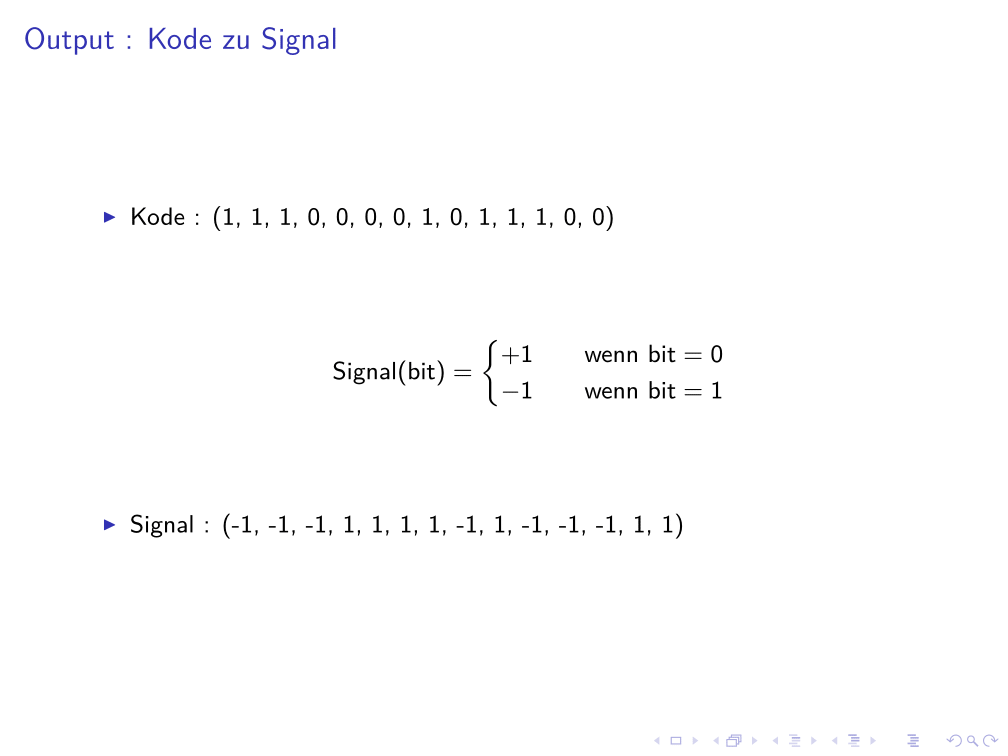
\includegraphics[width=0.7\textwidth]{abbildungen/folie_kodierung_bit_zu_signal}}
	\caption{Folie mit der Abbildung der Kodebits zu den Signalpegeln}
	\label{abb:folie_bit_zu_signal_abbildung}
\end{figure}
% Punktierung
Abbildung~\ref{abb:folie_punktierung} zeigt die Folie der Punktierung. Auf dieser wird die Punktierung des Signals, d.h. das Entfernen von Signalwerten (definiert durch die Punktierungsmatrix) dargestellt. Dabei wird, neben dem originalen Signal und der Punktierungsmatrix, das punktierte Signal dargestellt, wobei zunächst die punktierten Signalwerte, d.h. die entfernten Werte, durch Asterisk-Symbole ($\ast$) ersetzt werden. Diese Darstellung dient als visueller Zwischenschritt für das anschließende tatsächlich punktierte Signal, bei dem die punktierten Werte fehlen, was dem Rückgabewert der Funktion entspricht.
\begin{figure}[th]
	\centering
	\fbox{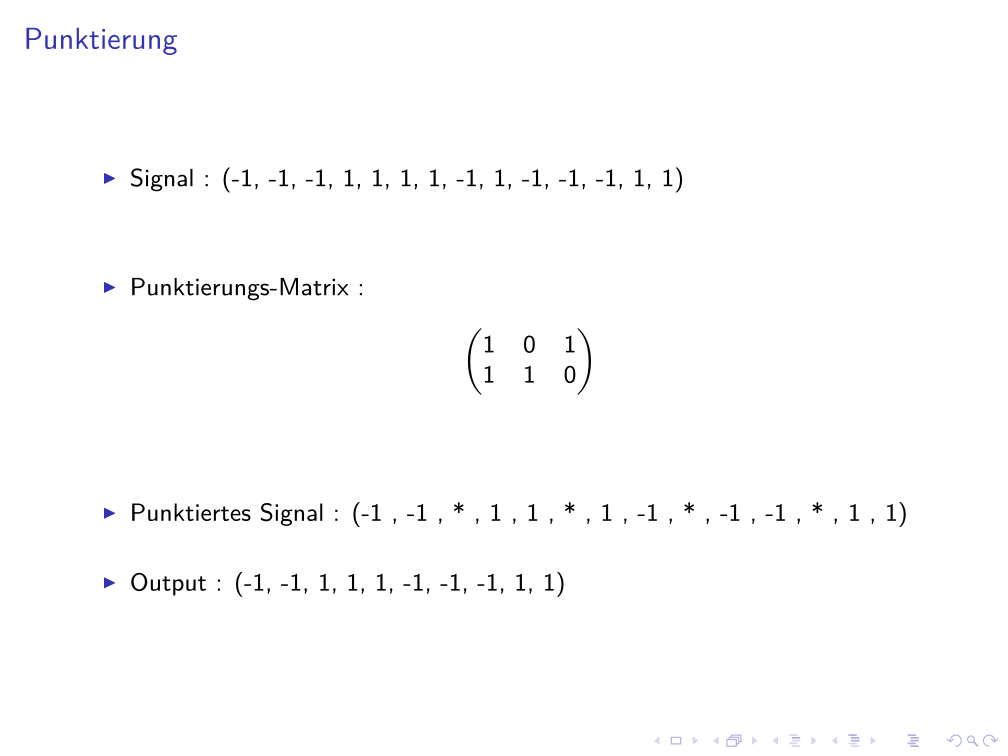
\includegraphics[width=0.7\textwidth]{abbildungen/folie_kodierung_punktierung}}
	\caption{Folie mit Punktierung}
	\label{abb:folie_punktierung}
\end{figure}
\FloatBarrier
\section{Dekodierung}
\label{kapitel:visualisierung_dekodierung}
% allg. Informationen
Bei der Dekodierung befinden sich ebenfalls, wie bei der Kodierung, allgemeine Informationen des Faltungskodierers auf den ersten Folien.
\\
% Depunktierung
Abbildung~\ref{abb:folie_depunktierung} zeigt die Folie der Depunktierung. Auf dieser wird die Depunktierung des Signals, d.h. das Einfügen des Signalwerts 0 (definiert durch die Punktierungsmatrix), dargestellt. Die eingefügten 0-Werte sind zur leichteren visuellen Erkennung farblich hervorgehoben.
\begin{figure}[th]
	\centering
	\fbox{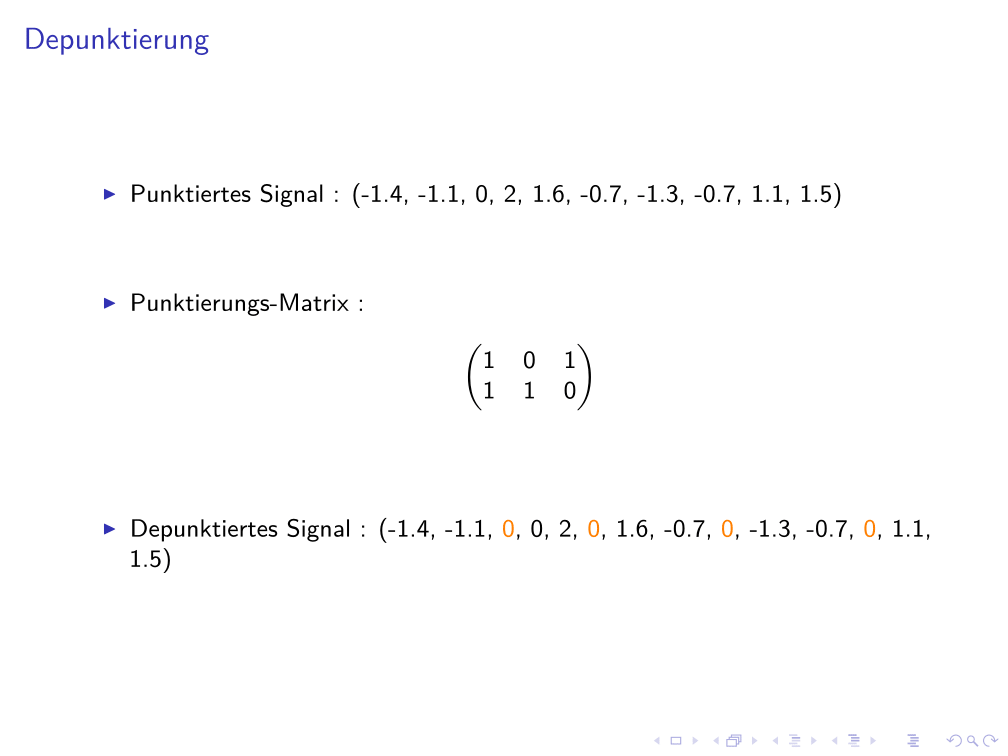
\includegraphics[width=0.7\textwidth]{abbildungen/folie_dekodierung_depunktierung}}
	\caption{Folie mit Depunktierung}
	\label{abb:folie_depunktierung}
\end{figure}
% Signal zu Kode
Als Input erhält die Dekodierung das Kodewort als kontinuierliche Signalwerte, die möglicherweise durch Anwendung der \texttt{ApplyNoise}-Funktion verfälscht worden sind. Die soft decision Dekodierung verwendet zur Dekodierung zwar direkt diese Signalwerte, da aber sowohl die hard decision Dekodierung Bitwerte zur Dekodierung verwendet, als auch die Kanten des Trellis mit Bitwerten beschriftet sind, wird der Input, um konsistent zu bleiben, auf Bitwerte abgebildet. Die Folie der Abbildung der Signalwerte auf Bitwerte nach Gleichung~\eqref{eq:signal_zu_bit_abbildung} ist in Abbildung~\ref{abb:folie_signal_zu_bit_abbildung} zu sehen.
\begin{figure}[th]
	\centering
	\fbox{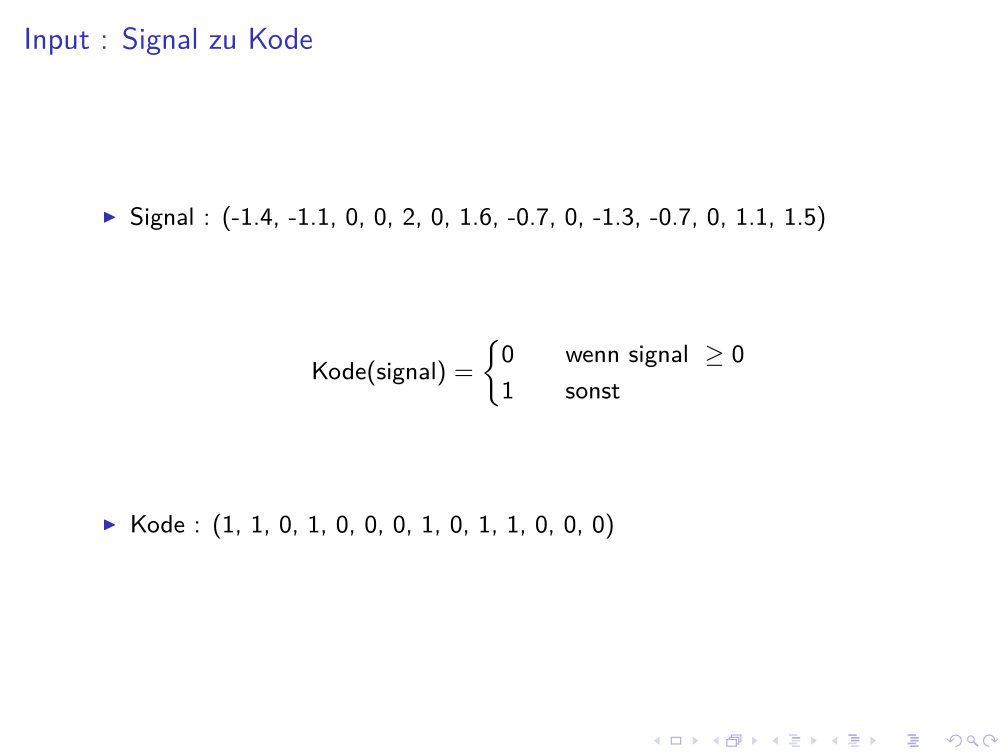
\includegraphics[width=0.7\textwidth]{abbildungen/folie_dekodierung_signal_zu_bit}}
	\caption{Folie mit der Abbildung der Signalpegel zu den Kodebits}
	\label{abb:folie_signal_zu_bit_abbildung}
\end{figure}
% Viterbi-Algorithmus
Anschließend folgt die Visualisierung des Viterbi-Algorithmus mithilfe des Trellis-Diagramms. In den farbigen Kreisen befinden sich die Metriken der Pfade, die zum jeweiligen Zustand führen. Zunächst werden, zur besseren Übersicht bei großen Diagrammen, jene Pfade entfernt, für die es eine bessere Alternative gibt. Es werden also jene Pfade entfernt, die bei der soft decision Dekodierung eine niedrigere Metrik bzw. bei der hard decision Dekodierung eine höhere Metrik besitzen. Dieser Schritt ist zwischen den Abbildungen~\ref{abb:folie_dekodierung_1} und \ref{abb:folie_dekodierung_2} zu sehen. Danach erfolgt Schritt für Schritt die Rekonstruktion der Nachricht mittels Backtracking. Der gewählte Pfad beim Backtracking wird farblich hervorgehoben. Die übrigen Pfade werden ausgegraut. Eine Folie während des Backtrackings wird in Abbildung~\ref{abb:folie_dekodierung_3} veranschaulicht. Am Ende befindet sich unter dem Trellis-Diagramm die farblich hervorgehobene dekodierte Nachricht, wie in Abbildung~\ref{abb:folie_dekodierung_4} dargestellt. Die einzelnen Zwischenschritte vermitteln dem Benutzer wie der Algorithmus funktioniert und wie sich die dekodierte Nachricht ergibt.
\begin{figure}[th]
	\centering
	\fbox{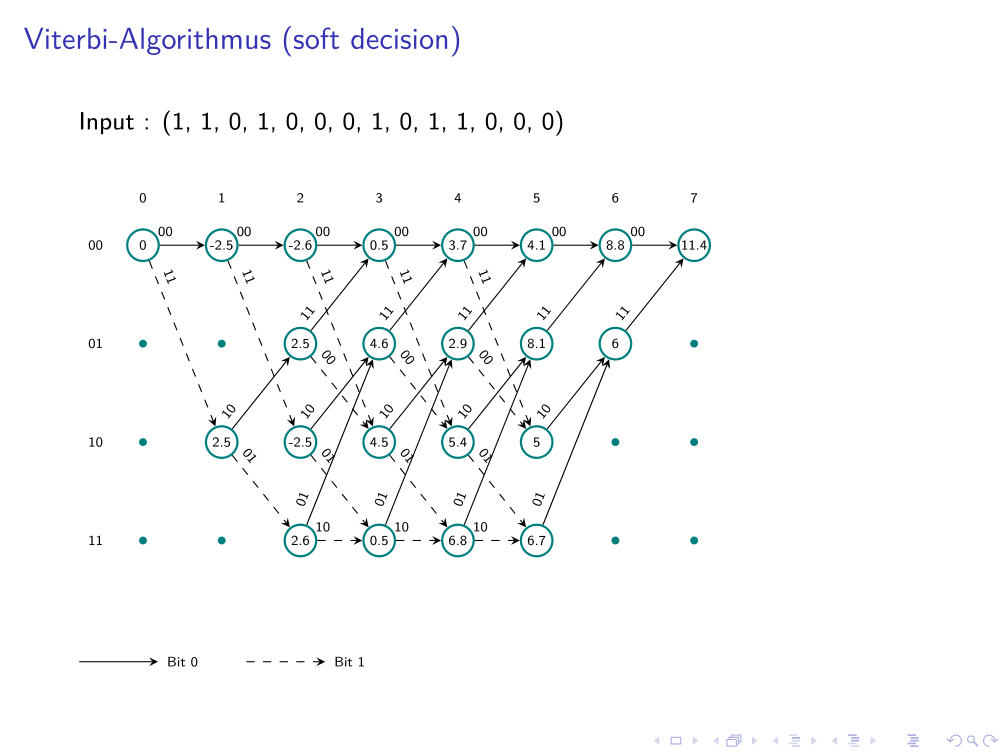
\includegraphics[width=0.7\textwidth]{abbildungen/folie_dekodierung_1}}
	\caption{Folie der soft decision Dekodierung und dem vollständigen Trellis}
	\label{abb:folie_dekodierung_1}
\end{figure}
\begin{figure}[th]
	\centering
	\fbox{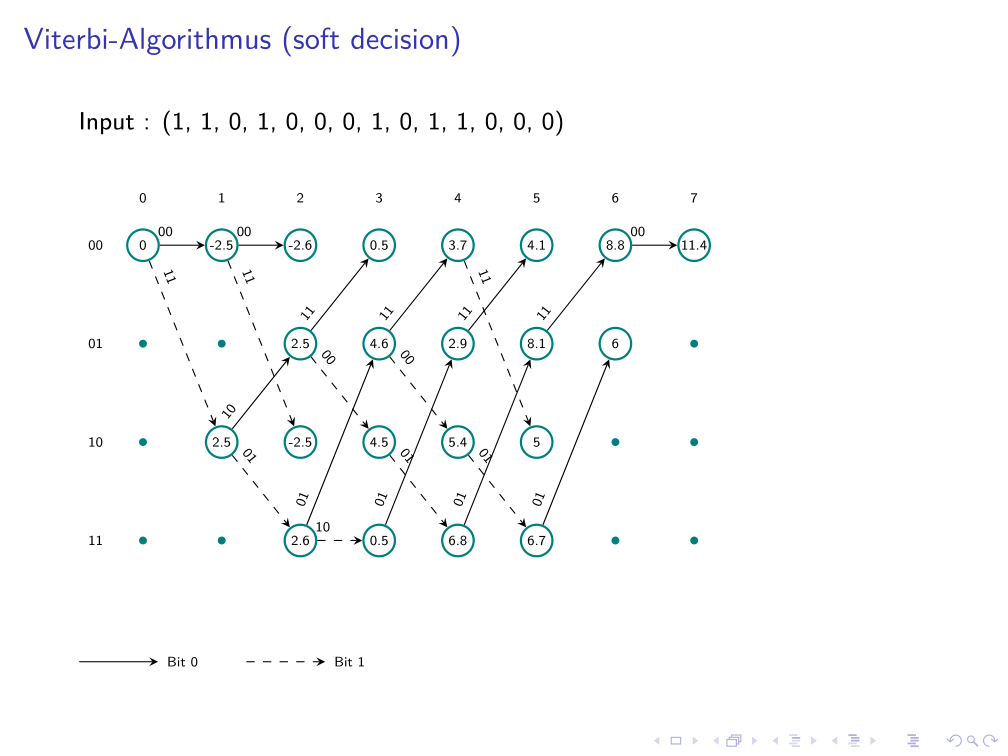
\includegraphics[width=0.7\textwidth]{abbildungen/folie_dekodierung_2}}
	\caption{Folie der soft decision Dekodierung und dem Trellis nach dem Entfernen einiger Pfade}
	\label{abb:folie_dekodierung_2}
\end{figure}
\begin{figure}[th]
	\centering
	\fbox{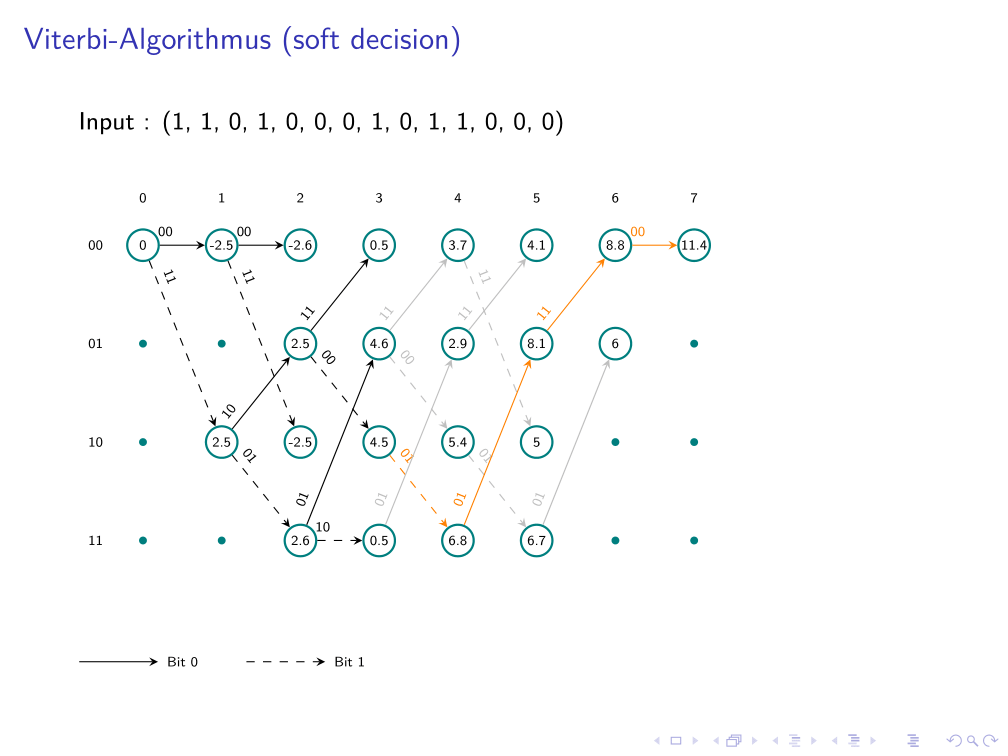
\includegraphics[width=0.7\textwidth]{abbildungen/folie_dekodierung_3}}
	\caption{Folie der soft decision Dekodierung im während dem Backtracking}
	\label{abb:folie_dekodierung_3}
\end{figure}
\begin{figure}[th]
	\centering
	\fbox{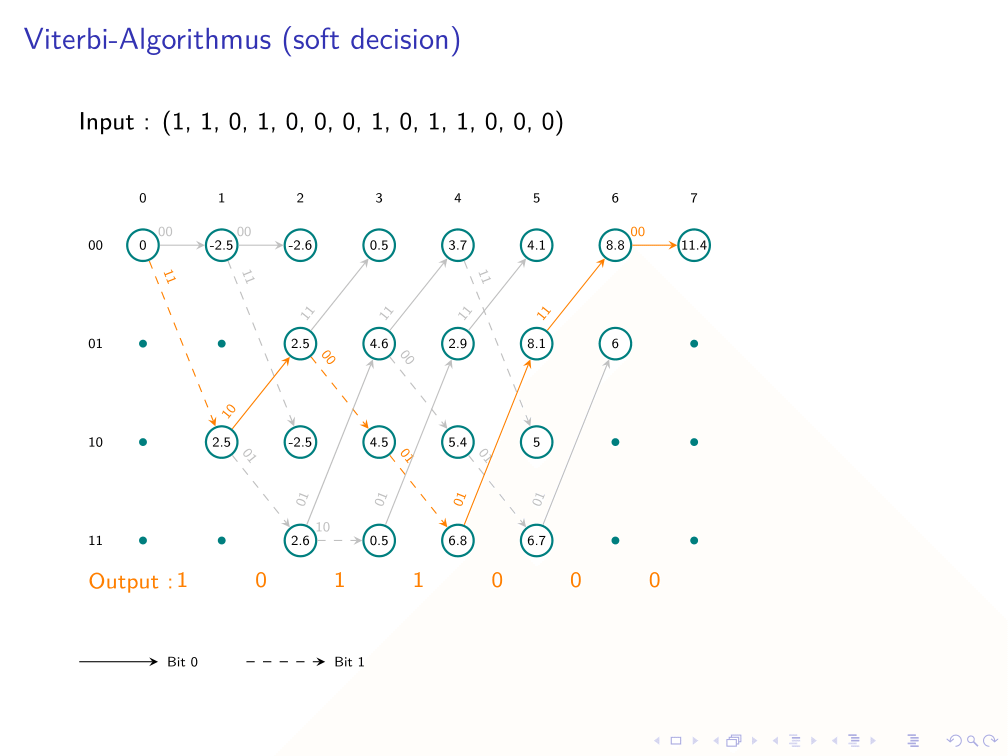
\includegraphics[width=0.7\textwidth]{abbildungen/folie_dekodierung_4}}
	\caption{Folie der soft decision Dekodierung mit der dekodierten Nachricht}
	\label{abb:folie_dekodierung_4}
\end{figure}

\section{Simulation}
\label{kapitel:visualisierung_simulation}
Auch die Simulationsfunktionen bieten durch den \texttt{visualize}-Parameter die Möglichkeit eine Visualisierung generieren zu lassen. Kapitel~\ref{kapitel:visualisierung_simulation_faltungskodierung} erläutert die Präsentation der Faltungskode-Simulation. Die Folien der Simulation verschiedener Varianten der Kanalkodierung, um diese vergleichen zu können, sind in Kapitel~\ref{kapitel:visualisierung_simulation_kanalkodierung} beschrieben.

\subsection{Faltungskodierung}
\label{kapitel:visualisierung_simulation_faltungskodierung}
Die folgenden Folien sind das Resultat der Ausführung der \texttt{ConvSimulation}-Funktion. Auf den ersten Folien sind, wie schon bei der Kodierung und Dekodierung, Informationen zum verwendeten Faltungskodierer angegeben.
\\
Anschließend folgt eine Folie mit den Eckdaten der Simulation, wie in Abbildung~\ref{abb:folie_simulation_f1} ersichtlich.
\\
Die nächste Folie, dargestellt in Abbildung~\ref{abb:folie_simulation_f2}, stellt ein Diagramm der Daten des erzeugten Dataframes dar. Die x-Achse entspricht dem Signal-Rausch-Verhältnis. Auf der y-Achse werden die gemessenen Bitfehlerraten aufgetragen. Es ist in diesem Beispiel sehr gut zu erkennen, dass die Fehleranzahl mit steigendem Signal-Rausch-Verhältnis abnimmt.
\\
Abschließend werden statistische Kennzahlen der Bitfehlerraten wie Minimum, Maximum, Median etc. auf der letzten Folie, wie in Abbildung~\ref{abb:folie_simulation_f3} zu sehen, aufgelistet. 
\begin{figure}[th]
	\centering
	\begin{subfigure}{0.48\textwidth}
		\centering
		\fbox{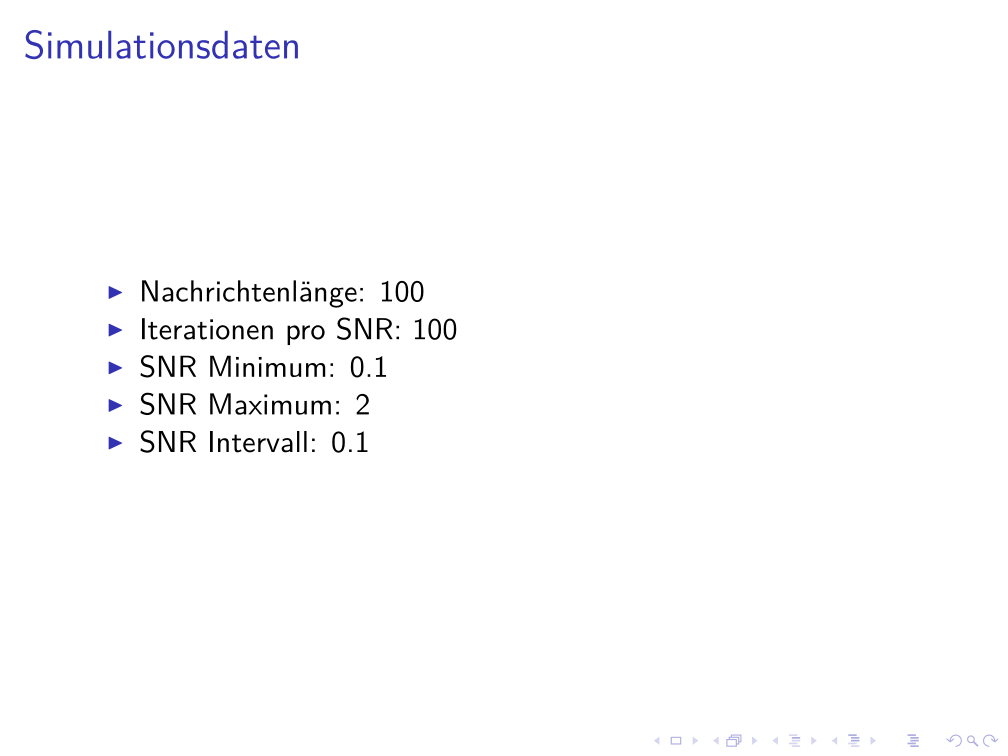
\includegraphics[width=0.99\textwidth]{abbildungen/folie_simulation_f1}}
		\caption{Folie mit Simulationseckdaten\\ \textcolor{white}{x}}
		\label{abb:folie_simulation_f1}
	\end{subfigure}
	\quad
	\begin{subfigure}{0.48\textwidth}
		\centering
		\fbox{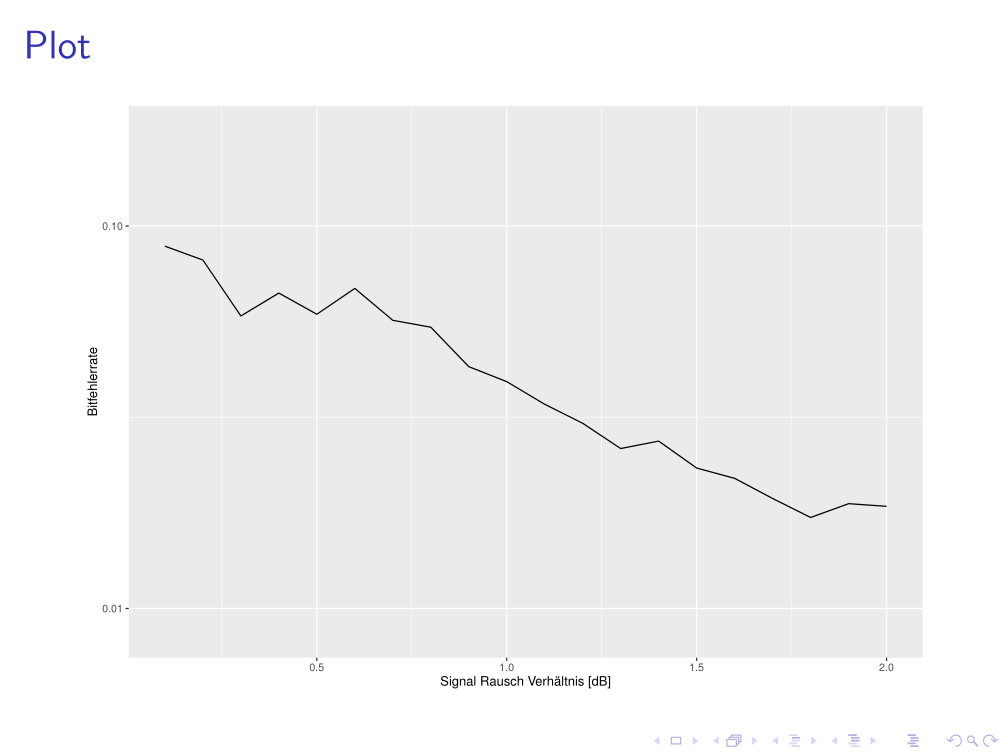
\includegraphics[width=0.99\textwidth]{abbildungen/folie_simulation_f2}}
		\caption{Folie mit Diagramm der Simulationsergebnisse}
		\label{abb:folie_simulation_f2}
	\end{subfigure}
	\par\bigskip
	\begin{subfigure}{0.48\textwidth}
		\centering
		\fbox{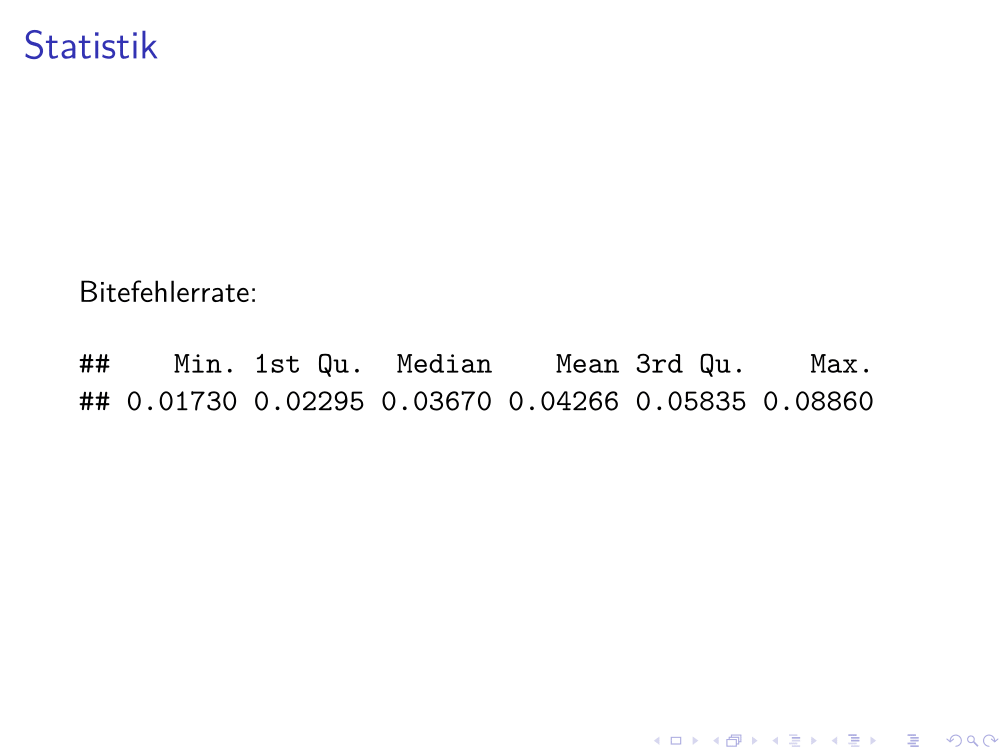
\includegraphics[width=0.99\textwidth]{abbildungen/folie_simulation_f3}}
		\caption{Folie mit Statistik der Bitfehlerraten}
		\label{abb:folie_simulation_f3}
	\end{subfigure}
	\caption{Folien der Faltungskodierungs-Simulation}
	\label{abb:folie_simulation_f}
\end{figure}

\subsection{Kanalkodierung}
\label{kapitel:visualisierung_simulation_kanalkodierung}
\begin{figure}[th]
	\centering
	\begin{subfigure}{0.48\textwidth}
		\centering
		\fbox{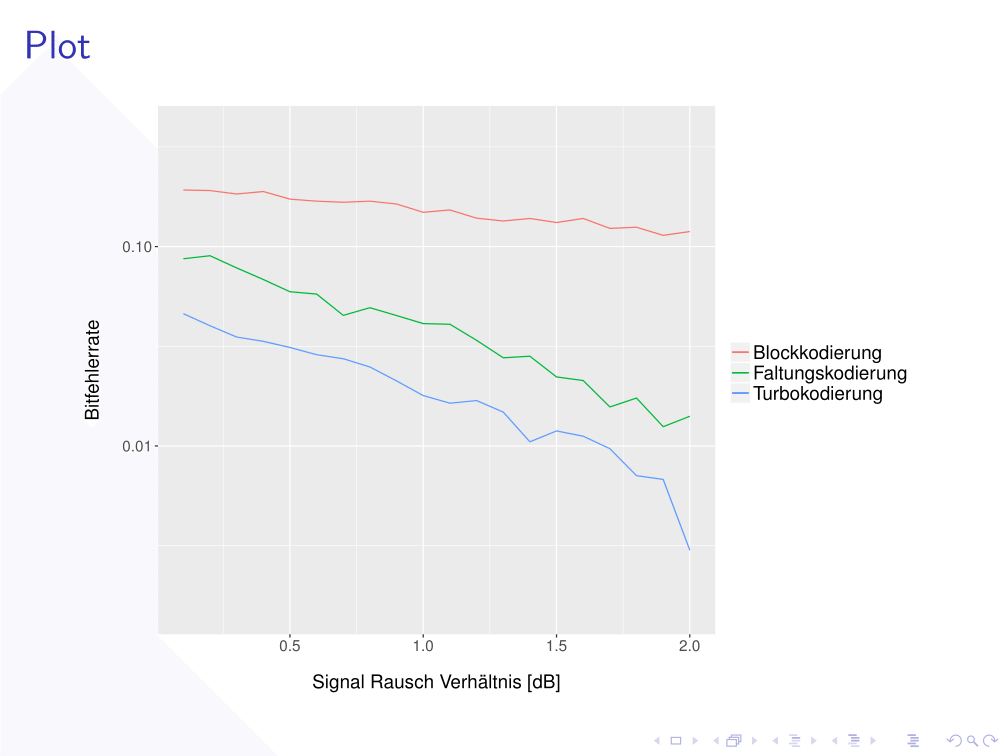
\includegraphics[width=0.99\textwidth]{abbildungen/folie_simulation_k1}}
		\caption{Folie mit Diagramm der Ergebnisse}
		\label{abb:folie_simulation_k1}
	\end{subfigure}
	\quad
	\begin{subfigure}{0.48\textwidth}
		\centering
		\fbox{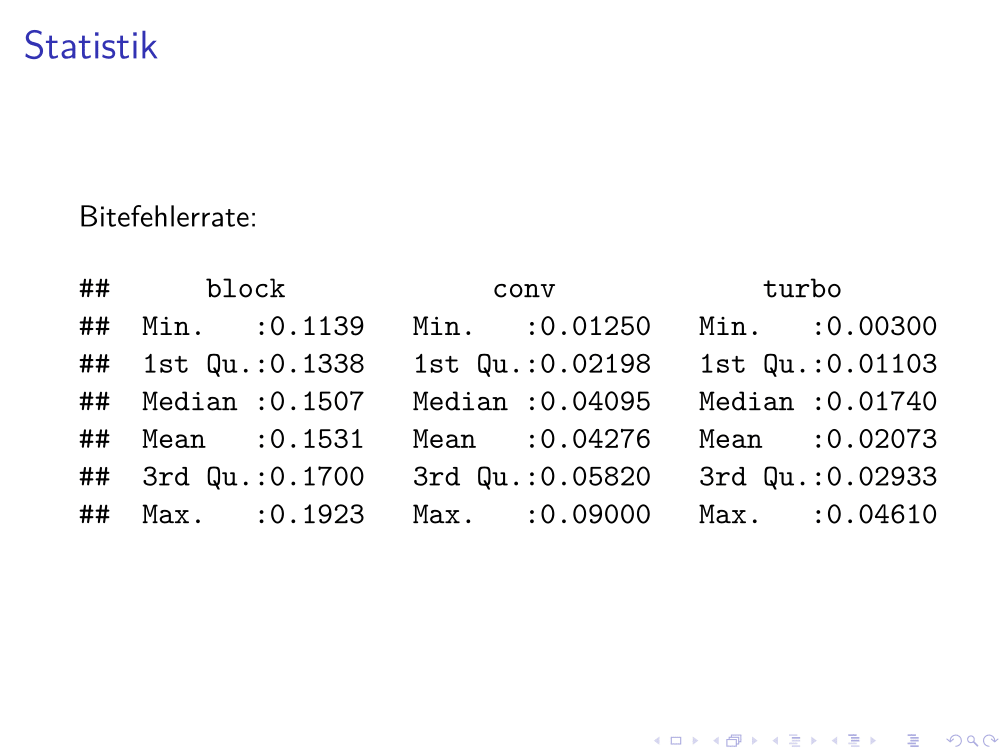
\includegraphics[width=0.99\textwidth]{abbildungen/folie_simulation_k2}}
		\caption{Folie mit Simulationsstatistik}
		\label{abb:folie_simulation_k2}
	\end{subfigure}
	\caption{Folien der Kanalkodierungs-Simulation}
	\label{abb:folie_simulation_k}
\end{figure}
Für einen Vergleich der im R-Paket implementierten Verfahren der Kanalkodierung kann die \texttt{ChannelcodingSimulation}-Funktion ausgeführt werden, deren Simulationsergebnisse ebenfalls dargestellt werden können. Zu Beginn der Kanalkodierungs-Visualisierungen werden auf einer Folie die Simulationseckdaten aufgelistet, wie es schon bei der Visualisierung der Faltungskodierungs-Simulation der Fall war.
\\
Abbildung~\ref{abb:folie_simulation_k1} zeigt die Folie mit dem Diagramm, in dem die Ergebnisse der drei Simulationen dargestellt werden und miteinander verglichen werden können. Die Art der Kodierung einer Kurve kann anhand der Farbe zugeordnet werden.
%\begin{figure}[th]
%	\centering
%	\fbox{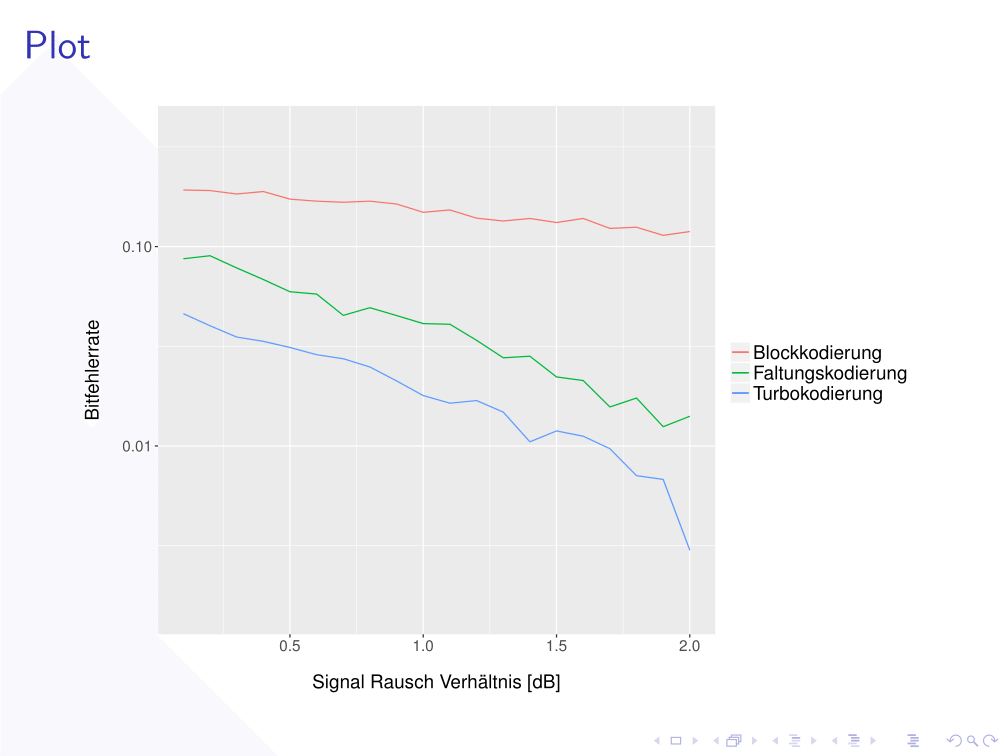
\includegraphics[width=0.7\textwidth]{abbildungen/folie_simulation_k1}}
%	\caption{Folie mit Diagramm der Ergebnisse der Kanalkodierungs-Simulationen}
%	\label{abb:folie_simulation_k1}
%\end{figure}
Wie auch schon in Kapitel~\ref{kapitel:visualisierung_simulation_faltungskodierung} befindet sich auf der letzten Folie eine Statistik der Bitfehlerraten. Dabei werden die Werte der verschiedenen Kanalkodierungs-Varianten gegenübergestellt. Abbildung~\ref{abb:folie_simulation_k2} zeigt ein Beispiel zur Statistik-Folie.
%\begin{figure}[th]
%	\centering
%	\fbox{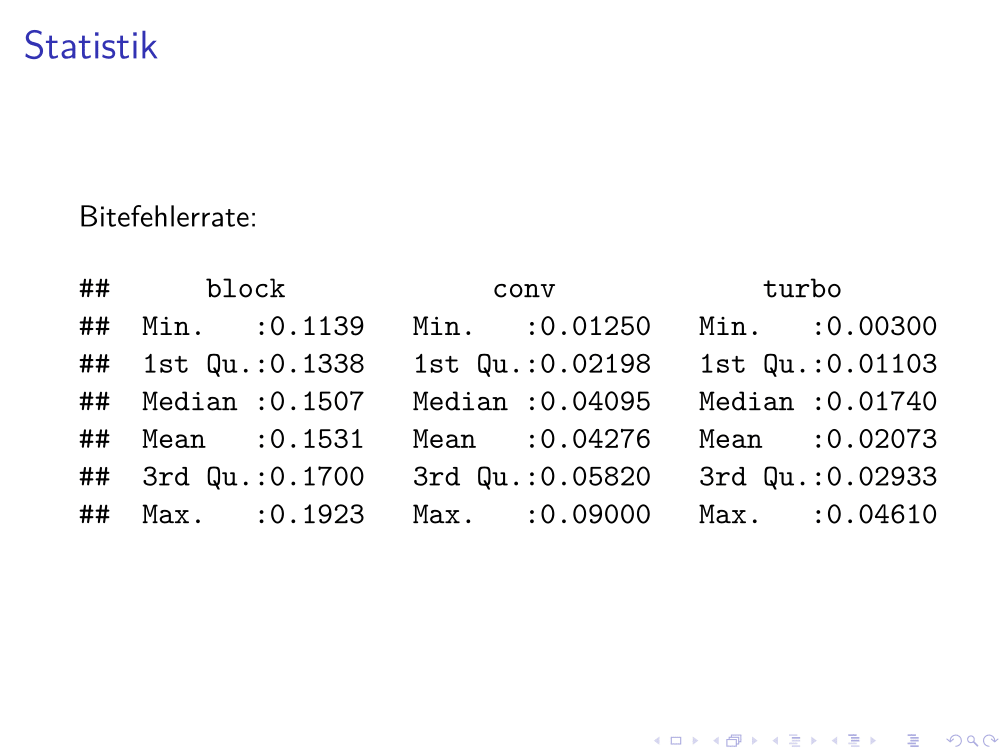
\includegraphics[width=0.7\textwidth]{abbildungen/folie_simulation_k2}}
%	\caption{Folie mit Simulationsstatistik}
%	\label{abb:folie_simulation_k2}
%\end{figure}